\section{Architecture} \label{Architecture}

\subsection{Architectural Constraints}

Constraints placed on the architectural decisions made are derived directly from the requirements listed in section \ref{Requirements}.

\subsubsection{Framework}
Section \ref{Technology Requirements} specifies that the Flutter SDK must be used for the implementation of Invite Only. Additionally, services provided by the Firebase platform are also listed as requirements. As a consequence, the architecture of the system will need to cater for the integration of a Flutter application with the required Firebase services.

\subsubsection{Language}
As a result of the framework constraints mentioned above, the dart programming language will have to be used to implement the system. This places additional constraints on any packages that are used, which will have to be published on \url{https://pub.dev} to be included as dependencies of the application.

\subsubsection{Database}
Since Firebase's Cloud Firestore will be used for the storage of data, the architecture must cater for constraints imposed by the usage of a NoSQL database. This includes catering for a lack of referential integrity and data structured in the form of JSON collections and documents.

\subsubsection{Timescales}
The timescale provided to implement the Invite Only system is minimal. As such, the architectural design must allow, where possible, for existing tools and technologies to be used. Lastly, should the system not be entirely complete within the time constraints, the time spent on development must yield at least some working software.

\newpage

\subsection{Architectural Design}

On a high level, Invite Only uses the 2-tier architectural pattern encompassed by most applications using the Firebase platform. In contrast to a traditional 3-tier approach, whereby there is a communication layer between the mobile app and the backend service, in the 2-tier model mobile apps and Firebase both manipulate the data directly. Authentication and validation are specified as declarative rules in the Firebase web UI, with no need to write imperative code.

This approach was chosen, in accordance with requirements, to take advantage of the rapid development of a backend service, real-time data synchronization across multiple devices and automatic scaling benefits of using Firebase. Figure \ref{fig:overview_firebase} shows this high level approach diagrammatically.

\begin{figure}[H]
  \centering
  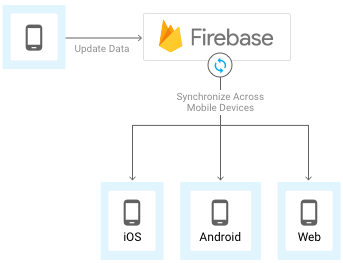
\includegraphics[width=1.0\textwidth]{documentation/software_requirements_specification/architecture/overview_firebase.png}
    \footnotesize \url{https://cloud.google.com/solutions/mobile/mobile-app-backend-services}
  \caption{2-tier Architecture Overview}
  \label{fig:overview_firebase}
\end{figure}

On a slightly more refined level, a plugin-oriented architectural approach is used, with the Invite Only application making use of a variety of self-contained plugins, usually in the form of dart packages or Flutter plugins, when it is possible and logical to black box specific functionality.

Some of these self-contained plugins will be developed in conjunction with, but independent from, the Invite Only platform whilst others are provided by third parties. One service that will be developed internally is the \href{https://pub.dev/packages/rsa\_identification}{rsa\_identification package}, used for decoding and providing South African identification details from documents such as Driver's licenses and Smart ID's. Importantly, the specifications of independent plugins will not be detailed in this document, only their interactions.

As for the Invite Only application itself, component-based development will be used to support separation of concerns with respect to the wide-ranging functionality available throughout the application. Components, or subsystems, will be implemented in the form of libraries and have already been mentioned in previous sections - they include the User, Space, Access and Invite libraries.

Figure \ref{fig:invite_only_component} illustrates how Service-Oriented Architecture and Component-Based Development are applied within the context of Invite Only by showing components, provided and required interfaces, ports, and relationships between them.

It is noteworthy that there are some obvious internal library dependencies not shown in figure \ref{fig:invite_only_component}. For example, all libraries are dependant on the User Library to determine the currently authenticated user. These internal interfaces are omitted from the diagram so as not to over-complicate and detract from more noteworthy dependencies.

Finally, each of the libraries (Access, User, Space and Invite) will adhere to a layered architecture consisting of a UI layer, a Presentation/Logic layer and a Domain layer. The UI and Presentation/Logic layers are representative of the commonly used Model-View-ViewModel pattern; however, in our case, Blocs (Business Logic Objects) will be used in the place of ViewModels. This architectural pattern, portrayed by figure \ref{fig:library_architecture}, was chosen to ensure maintainable, testable and performant code.

\begin{figure}[H]
  \centering
  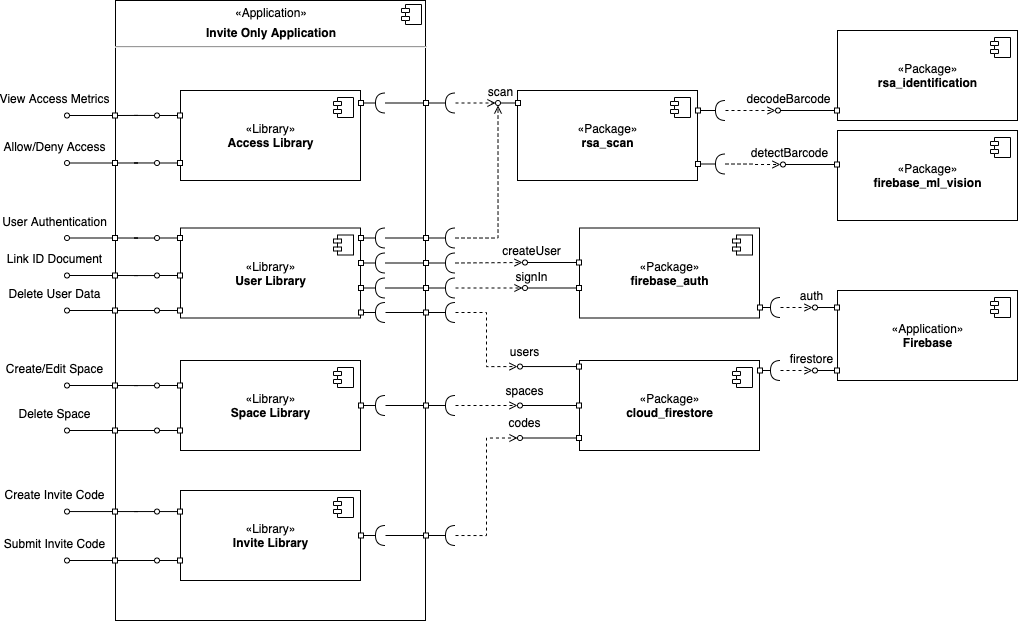
\includegraphics[width=1.0\textwidth]{documentation/software_requirements_specification/architecture/component_diagram.png}
  \caption{Component Diagram}
  \label{fig:invite_only_component}
\end{figure}

\begin{figure}[H]
  \centering
  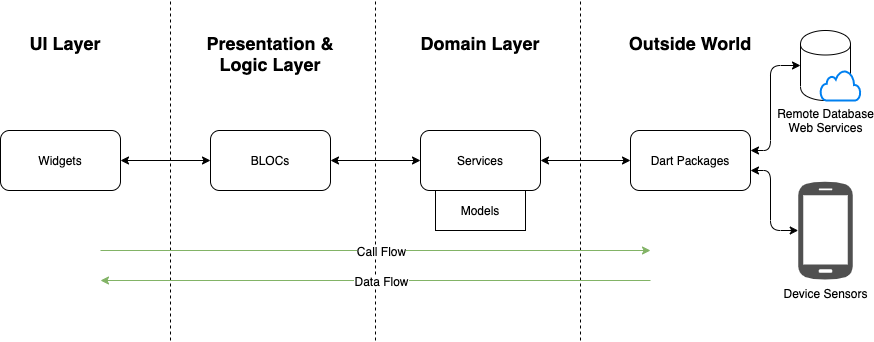
\includegraphics[width=1.0\textwidth]{documentation/software_requirements_specification/architecture/library_architecture.png}
  \caption{Layered Library Architecture}
  \label{fig:library_architecture}
\end{figure}

\newpage

\subsection{Deployment Model}

Packages, although they are independent, are compiled and packaged along with the application - as a result, the deployment diagram shown in figure \ref{fig:deployment_model} is relatively straightforward and quite different to the libraries and subsystems described from an architectural perspective. This is because the Flutter SDK compiles the source code, written following our architecture, ahead-of-time to native code, which looks very different to our architecture.

In any case, once compiled the applications exists as two executable artifacts - specifically, an APK file and an IPA file. The APK file is deployed to any device running the Android operating system while the IPA file is deployed any device running the iOS operating system. Following installation on a device, the application communicates with services deployed on the Firebase application server using HTTPS.

\begin{figure}[H]
  \centering
  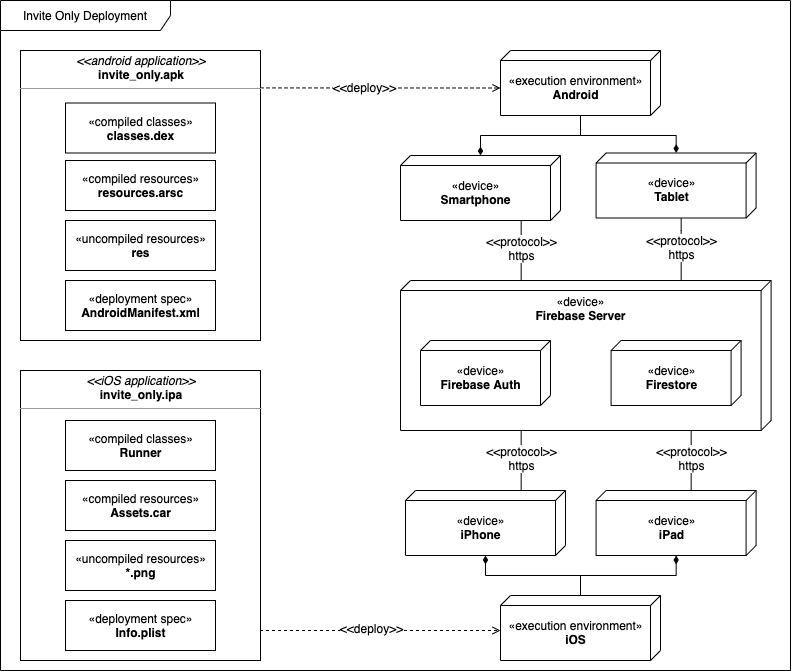
\includegraphics[width=0.9\textwidth]{documentation/software_requirements_specification/architecture/deployment_model.png}
  \caption{Deployment Model}
  \label{fig:deployment_model}
\end{figure}